\chapter{ENFOQUE DE MERCADO.} %(((
A continuación se detallan las categorías de activos en las que se encontró mercado disponible para la comparación entre activos.
\begin{itemize}
	\item Tanque para aire comprimido.
	\item Polipasto eléctrico. 
	\item Bombo batidor/mezclador para confitería.
	\item Compresor horizontal.
	\item Secador de aire refrigerado.
	\item Compresor de aire.
\end{itemize}
En las categorías en las que no se encontró mercado, 
se procede directamente a realizar el análisis de demérito por edad sobre el valor de factura.
% en la sección 

\section{} % (((

\subsection{--- Enfoque de Mercado. ---} % (((
\begin{figure}[hbtp!]
	\centering
	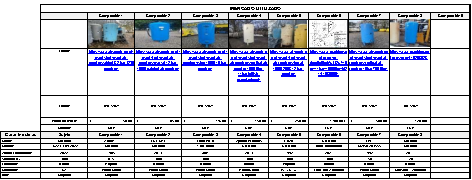
\includegraphics[width=  \linewidth, page = 1]{../0.imagenes/CAP_11/cap_11}
\end{figure}
Se procede con el análisis estadístico para determinar la significancia de un modelo de regresión lineal. \\ 
Se toma un valor de confianza del \(90\%\).
% )))

\subsection{--- Planteamiento ---} % (((
El modelo de regresión lineal planteado tiene las sig. variables:
\begin{table}[hbtp!]
	\centering
	\begin{tabular}{r @{: \hspace{5mm}} l}
		\hline 
		X1 &  \\ \hline
		X2 &  \\ \hline
		X3 &  \\ \hline
		Y  &  \\ \hline
	\end{tabular}
\end{table}
% )))

\subsection{--- Matriz de Dispersion ---} % (((
Se obtienen los coeficientes de correlacion lineal individuales entre las características del activo y se interpretan.
\begin{center}
  \begin{tabular}{|p{11cm}|p{5cm}|}
    \hline
    Gráfica & Interpretación. \\ \hline 
    \begin{minipage}{\textwidth}
    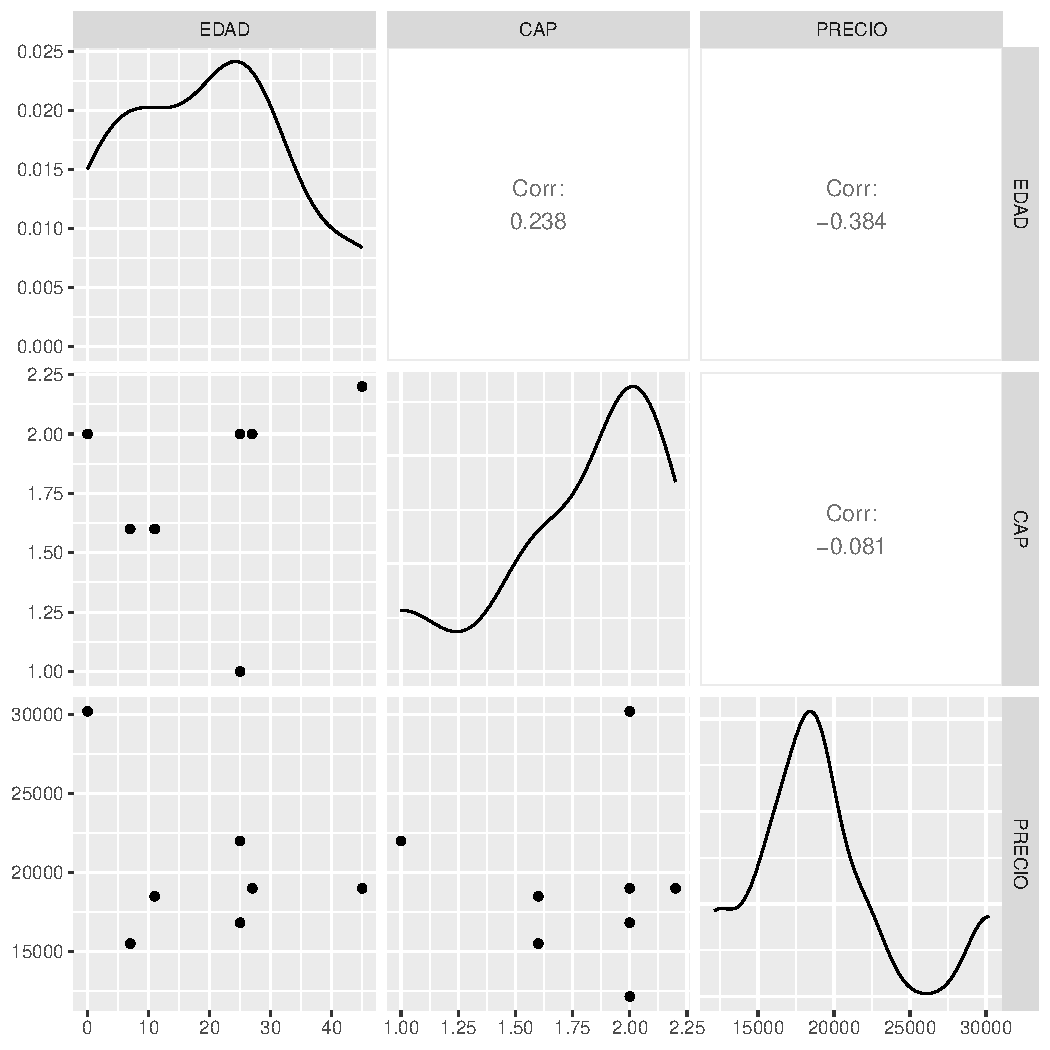
\includegraphics[width= 0.6 \linewidth, page=1]{../0.documentos/ANALISIS_R/1/Rplots}
    \end{minipage} 
		& 
		El coef. de corr. de Pearson obtenido en todos fue menor al \(60\%\). \newline 
		Es decir, NO hay una correlación lineal individual entre cada una de las características (\(X_i\))
		con sus precios (\(Y\)).
\end{center} 
% )))

\subsection{--- Modelo de Regresión ---} % (((
Se obtiene el Modelo de Regresión Lineal Estimado con los datos obtenidos.
\begin{equation}
	Y = 
	\label{eq:1}
\end{equation}
% )))

\subsection{--- Tabla ANOVA ---} % (((
Tomamos el valor de confianza para el análisis estadístico de un \(95\%\). (\(\alpha =0.1\)). \\ 
Se realiza la tabla ANOVA.
\begin{center}
  \begin{tabular}{|p{2cm}|p{2cm}|p{2cm}|p{2cm}|l|}
    \hline 
    Fuentes de Variación  & Suma de Cuadrados & Grados de Libertad & Cuadrados Medios & F\\ \hline 
    Regresión           &  &           &        &  \\ \hline 
    Error               &  &           &        &  \\ \hline 
    Totales             &  &           &        &  \\ \hline 
  \end{tabular}
\end{center} 
Se usará el valor \(F\) para determinar la significancia del modelo.
% )))

\subsection{--- Prueba de Significancia del Modelo ---} % (((
Se obtiene el coef. de corr. lineal de Pearson
\begin{table}[hbtp!]
	\centering
	\begin{tabular}{|p{2cm}|p{2cm}|p{10cm}|}
		\hline 
		\(r ^ 2\) &  \\ \hline
	\end{tabular}
\end{table}
Se comprueba la significancia del modelo con el estadístico \(F\) de la tabla ANOVA.
\begin{center}
  \begin{tabular}{|l|p{11cm}|}
    \cline{1-2}
    \multicolumn{2}{|c|}{Hipótesis}\\ \cline{1-2}
		\multicolumn{2}{|l|}{\(H_0:\) El modelo no es significativo (\(p> \alpha\)).} \\ 
		\multicolumn{2}{|l|}{\(H_a:\) El modelo es significativo (\(p< \alpha\)).} \\ \cline{1-2}
    Estadístico de Prueba & \(50.83\).\\ \cline{1-2} 
    Región de Rechazo & \((0, \alpha )\).\\ \cline{1-2} 
    Valor \(p\) & \(1.7e-14\).\\ \cline{1-2} 
    Conclusión & Se tiene que \(p<\alpha\), por tanto se rechaza \(H_0\). Es decir, el modelo es significativo.\\ \cline{1-2} 
  \end{tabular}
\end{center} 
% \textbf{Conclusión:} Se rechaza el modelo lineal para determinar el precio del activo, dado que no es significativo. \\ 
% Por tanto, se procede con el análisis de 
% \textbf{Conclusión:} Se acepta el modelo lineal para determinar el precio del activo a un \(95\%\) de confianza. \\ 
% Los datos de el activo son los siguientes:
% \begin{table}[hbtp!]
	% \centering
	% \begin{tabular}{|p{2cm}|p{2cm}|}
		% X0 & \\ \hline 
		% X0 & \\ \hline 
		% X0 & \\ \hline 
		% X0 & \\ \hline 
	% \end{tabular}
% \end{table}
% Así, el precio del activo aplicado al modelo lineal \eqref{eq:1}, se obtiene 
% \(Y = \).
% )))

% )))

% )))

